\documentclass[draftclsnofoot, onecolumn, compsoc, 10pt]{IEEEtran}

\title{\huge Software Requirements Specifications}

\author{Oregon State University\\CS 461\\2016-2017\\\\Prepared By:\\Nic Desilets, James Stallkamp,\\and Nathaniel Whitlock}

\usepackage{titling}

\usepackage[margin=0.75in]{geometry}

\usepackage{graphicx}

\linespread{1.0} % 1.0 = single, 1.3 = 1.5, 1.6 = double

\parindent=0.0in

\parskip=0.2in

\begin{document}
\begin{titlingpage}
    \maketitle 
\end{titlingpage}

\tableofcontents
\pagebreak

% Section One
\section{Introduction}

\subsection{Purpose}
The purpose of this document is to define the primary objective and details of the toolkit.
This document will contain guidelines that describe the purpose, features, general design, interactions with Oracle 12c database, and the constraints that the performance analysis toolkit must operate within.
The target audience for this document includes any relevant stakeholders as well as any Database Administrator (DBA) or software developer that works with Oracle database 12c in any capacity.


\subsection{Scope}
The main purpose of this toolkit is primarily to assist with collecting and visualizing performance metrics when running database queries.
By doing so, this toolkit will allow us to benchmark database performance based on different configuration schemes in order to find the best solution.
Some of the configuration schemes will include modifying memory management, experimenting with varying degrees of parallelism, and altering database table partitioning. 

The primary performance metric that the toolkit will be measuring is the Performance Efficiency Index (PEI), which is database time divided by wall clock time, in order to better gauge query efficiency.
A higher PEI ratio (e.g. more database time spent per real world elapsed time) indicates higher database query efficiency.
Another useful metric that this toolkit will monitor is real world elapsed time which ultimately determines the perceived responsive of queries made against the database.

\subsection{Definitions, Acronyms, Abbreviations}

\bgroup
\def\arraystretch{1.5}
\resizebox{\textwidth}{!}{  
\begin{tabular}{| l | l |} % centered columns (4 columns)
\hline
\bf{Term} & \bf{Definition}\\ [0.5ex] 
\hline
Command Line Interface (CLI) & A application which provides a means of interacting with a computer program by entering lines of text \\ [0.5ex]
\hline
Central Processing Unit (CPU) & The physical processor(s) in the machine that executes instructions. \\ [0.5ex]
\hline
Database & Software which stores information in an organized, easy to access manner \\ [0.5ex]
\hline
Database Administrator (DBA) & Ensures availability, reliability, performance, security, and scalability of database systems \\ [0.5ex]
\hline
Database Time & The amount of real world time the database spends consuming CPU resources \\ [0.5ex]
\hline
Enterprise Manager (EM) & A set of web-based tools aimed at managing software and hardware produced by the Oracle company  \\ [0.5ex]
\hline
Gigabyte (GB) & A multiple of the storage unit byte, composed of $1024^3$ bytes of memory \\ [0.5ex]
\hline
HP Inc. (HP) & An American multinational information technology company headquartered in Palo Alto, California \\ [0.5ex]
\hline
Performance Efficiency Index (PEI) & Wall clock time divided by database time. Indicates database query efficiency \\ [0.5ex]
\hline
Random Access Memory (RAM) & Computer memory where any byte of storage can be accessed without touching the preceding bytes \\ [0.5ex]
\hline
Software Developer & Performs research, design, implementation, and testing of software products \\ [0.5ex]
\hline
Stakeholder & Anyone who does not fall under the role of database administrator or developer but is otherwise directly or indirectly involved \\ [0.5ex] 
\hline
Terabyte (TB) & A multiple of the storage unit byte, composed of $1024^4$ bytes of memory \\ [0.5ex]
\hline
Virtual Private Network (VPN) & A method of providing encrypted remote access to a remote computer over the internet \\ [0.5ex]
\hline
Wall clock time & Real world elapsed time \\ [0.5ex]
\hline
\end{tabular}
}
\egroup

\subsection{References}
IEEE.   IEEE Std 830-1998 IEEE Recommended Practice for Software Requirements Specifications. IEEE Computer Society, 1998.

\subsection{Overview}
The second section of this document, Overall Description, gives an overview of software dependencies, the intended function, characteristics, constraints, and assumptions of the toolkit.
This section is more geared towards general stakeholders given that it is more of a high level examination of the toolkit.
The third section of this document, Specific Requirements, is primarily intended for database administrators and software developers who are familiar with the technical aspects and relevant terminology of this toolkit.
These two sections are both designed to give a comprehensive overview of the toolkit to two different target audiences, one high level and one low level.

% Section Two
\section{Overall Description}

\subsection{Product Perspective}
The toolkit itself is not designed to be a standalone software application that runs independently of other software systems.
Rather, it is a component that is designed to integrate specifically with Oracle 12c in order to give DBA's and software developers quantitative metrics and information with respect to different database configurations.
The toolkit will be a compressed folder which will house many SQL scripts each serving it's own utility function.
Together these scripts will comprise a set of tools which would we will make available to DBA's and other senior level software engineers.

%% Begin subsubsection
\subsubsection{System Interfaces}
The primary system interfaces are Oracle Database 12c and Oracle Linux 7.
This toolkit will interact with an Oracle Database 12c instance to gather performance metrics from the database itself.
Additionally, the toolkit will be able to make system calls to Oracle Linux 7 in order to gather any other necessary metrics information relating to the systems processes.

\subsubsection{User Interfaces}
The user interface of the toolkit will be a command line interface in which the user can define parameters and execute commands that are supported by the toolkit.
The minimum required screen format must at least support a standard 80 character width by 24 character long terminal.

\subsubsection{Hardware Interfaces}
The toolkit is purely software based and does not involve any specific piece of hardware.
Since the toolkit is comprised of SQL scripts it will be executed by a system which is already configured. 

\subsubsection{Software Interfaces}
This toolkit is intended to be used with Oracle Database 12c running in an Oracle Linux 7 environment.
The required system software and additional supporting applications specifications are listed below:

\begin{itemize}
	\item Oracle Linux 7
	\begin{itemize}
		\item Mnemonic: OL7
		\item Version: 7.2
        \item Source: Oracle
	\end{itemize}
	\item Oracle Database 12c Enterprise Edition
	\begin{itemize}
		\item Mnemonic: 12c
        \item Version: 12.1.0.2.0
        \item Source: Oracle
	\end{itemize}
    \item Oracle Enterprise Manager Database Express 12c
	\begin{itemize}
		\item Mnemonic: EM
        \item Version: 12.1.0.2.0
        \item Source: Oracle
	\end{itemize}
   	\item Oracle SQL Developer
	\begin{itemize}
		\item Mnemonic: N/A
        \item Version: 4.1.5.21
        \item Source: Oracle
	\end{itemize}
    \item Command Line Interface
	\begin{itemize}
		\item Mnemonic: CLI
        \item Version: 3.8.13
        \item Source: Linux
	\end{itemize}
\end{itemize}


\subsubsection{Communications Interfaces}
There will be no communication interfaces that our toolkit will need to take into account any communication interface or network protocols.
The toolkit will be a series of scripts that will act as an instruction set for a previously configured system.

\subsubsection{Memory constraints}
The toolkit we will be developing will consist of a collection of SQL scripts, there are no inherent memory constraints. 

\subsubsection{Operations}
There will be only one mode of operation within the user organization which will be DBA level access.
Most of the periods operation will be ran in the background. Initially the user will configure the execution parameters and supply a query, then the system will take over the processing until the results are returned.
There will be no data processing or support functions and our toolkit will have no inherent backup or recovery functions.

\subsubsection{Site Adaptation Requirements}
There will be no site specific requirements for the use of the toolkit.
It will be available to anyone who chooses to download it in order to monitor the performance of there system during query execution.
%% End subsubsection

\subsection{Product Functions}
The overall functionality of this toolkit can be divided into four specific components.
Each one of the components works in concert to generate the performance metric report. These components are as follows:

%% Begin subsubsection
\subsubsection{Querying the Database}
This component will serve as the vehicle in which the user is able to submit a properly formatted SQL query against the database instance. 

\subsubsection{Modify Database Parameters}
This component will allow for the modification of system specific setting in order to optimize query performance.
We will use this to change settings within the Oracle 12c environment to increase processing efficiency.

\subsubsection{Gather System Metrics}
This component will use the dynamic performance views which are native to the Oracle 12c instance to monitor performance specifications during the execution of the provided query. 
Additionally, this component will make system calls out to the host operation system to isolate process time information that will be used as a performance metric. 

\subsubsection{Generate Performance Report}
This component will compile all of the system performance metrics which have been evaluated into a raw data report. This report can then be utilized by the users to create a visual report.
%% End subsubsection

\subsection{User Characteristics}
The users of our toolkit will be Senior level software developers that are writing queries on a server.
These users will have experience writing queries and interacting with a database.
These users should be proficient in one or more of SQL, Oracle 12c specifics, Python, shell scripting, Unix system calls, or parallel execution.
Users will have some level of formal technical education but this could vary from some college experience to doctorates.  

\subsection{Constraints}
The experiments that we will run will be limited to a specific machine, that machine will have 16 real cores, 500GB of memory and 5 TB of storage.
The software package that we create  will be able to run on any machine that can support Oracle SQL.
There will be no regulatory polices, audit functions, safety or security considerations within the scope of the toolkit.

\subsection{Assumptions and Dependencies}
In developing the performance evaluation toolkit we will be assuming that the scripts will be run on an Oracle SQL database.
The development of the toolkit will rely on a few specific factors which include:
\begin{itemize}
	\item Our computers must be connected to the local HP network to access the test database instance
    \begin{itemize}
    	\item Due to company firewall, outside access to the network is not possible without VPN
    \end{itemize}
	\item Access to physical location limited
    \begin{itemize}
    	\item Corvallis site limited to HP employees and contractors only, so an escort is needed
    \end{itemize}
	\item No access to server room
    \begin{itemize}
    	\item If the database goes down we have no access and must rely on HP counterpart to assist
    \end{itemize}
\end{itemize}

\subsection{Apportioning of Requirements}
Refer to the Gantt chart appended to the final page of this document.

\subsection{Toolkit Environment}
%<figure/diagram of users interacting with toolkit which interacts with database>
%Figure 1 - Toolkit Environment
The toolkit environment is comprised of four entities: Users which can be DBAs and software developers, the toolkit itself, the Oracle 12c database, and the host operating system that contains the database. Users interact with the toolkit by executing commands which can range from modifying various database parameters to executing queries on the database. While the database is the processing the queries, the toolkit will then begin monitoring critical performance metrics. The sources of the metrics can come from both the database itself and by polling the host operating system for more information about the database’s running processes.



% Section Three
\section{Specific Requirements}

\subsection{External Interfaces}
\begin{itemize}
	\item Input
    \begin{itemize}
    	\item Name: SQL Query.
        \item Description: A valid SQL that a user wants a performance report for.
        \item Source: Command line input from user. 
        \item Valid input: Any valid SQL statement.
    \end{itemize}
    \item Output
    \begin{itemize}
    	\item Name: System performance raw data report.
        \item Description: A raw data file of the performance statistics of the machine while running the input SQL query.
        \item Destination: A text file in the local directory.
    \end{itemize}
\end{itemize}

\subsection{Functions}
\begin{enumerate}
	\item The system shall accept an SQL query as input.
    \item The system shall fetch performance database tables to get statistics on the input query.
    \item The system shall organize the data and make recommendations on how to increase performance.
    \item The system shall output this data in into a data sheet.
\end{enumerate}

\subsection{Performance Requirements}
The system we are developing is a toolkit of scripts that will be easily attributable. 
This means the software can easily be installed and run on any number of machines simultaneously. 

\subsection{Logical Database Requirements}
Our software package will not be writing any data to a database.

\subsection{Design Constraints}
The only significant design constraint that we face is that our toolkit will be developed in Oracle SQL. 
That means that developing and using this software will have to be done on a machine that supports Oracle SQL.

\subsection{Standards Compliance}
Because our system is just a toolkit made up of scripts, there are not specific standards that we must comply with. 

\section{Software System Attributes}

\subsection{Reliability}
The reliability of this toolkit will be measured in it's ability to take valid SQL statements and generate a performance statistic report. 

\subsection{Security}
The toolkit will be available on a git hub repository that will be read-access only to the public. 
This will protect the integrity of the source code behind the toolkit. 
Individual users will be using the toolkit at their own risk, because they will already have full database access.
This toolkit does not pose any increased security risk. 

\subsection{Maintainability}
The toolkit will be organized so that each significant performance test will be in its own script file. 
These files will be well commented so that users can make changes as per their needs. 
The names of these scripts should be self explanatory and unique enough to distinguish their function from the name. 

\subsection{Portability}
The toolkit that is being created will be portable to any system that supports Oracle SQL 12c.
However this toolkit will not be portable to any other type of database.  

\subsection{Specific Requirements}

%% Begin subsubsection
\subsubsection{External Interface Requirements}
\begin{enumerate}
	\item User Interfaces: The user will interact with our software toolkit through the command line.
    	  Users will run these scripts on a SQL server to get a performance report.
     \item Hardware Interfaces: This software toolkit does not interact with hardware.
     \item Software Interfaces:
     \begin{itemize}
	 \item Oracle Linux 7
	 \begin{itemize}
		\item Mnemonic: OL7
		\item Version: 7.2
        \item Source: Oracle
	 \end{itemize}
	 \item Oracle Database 12c Enterprise Edition
	 \begin{itemize}
		\item Mnemonic: 12c
        \item Version: 12.1.0.2.0
        \item Source: Oracle
	 \end{itemize}
     \item Oracle Enterprise Manager Database Express 12c
	 \begin{itemize}
		\item Mnemonic: EM
        \item Version: 12.1.0.2.0
        \item Source: Oracle
	 \end{itemize}
     \item Oracle SQL Developer
	 \begin{itemize}
		\item Mnemonic: N/A
        \item Version: 4.1.5.21
        \item Source: Oracle
     \end{itemize}
     \item Command Line Interface
	 \begin{itemize}
		\item Mnemonic: CLI
        \item Version: 3.8.13
        \item Source: Linux
	 \end{itemize}
	 \end{itemize}
     \item Communications Interfaces: This toolkit will not interact with any communication or network protocols.
\end{enumerate}

\subsubsection{Functional Requirements}

\paragraph{Database Administrator User Class}
\begin{enumerate}
  \item The system shall accept an SQL query as input.
  \item The system shall fetch performance database tables to get statistics on the input query.
  \item The system shall organize the data and make recommend adjustments to increase performance.
  \item The system shall output this data in into a data sheet.
\end{enumerate}

\subsubsection{Performance Requirements}
The toolkit will be distributed across many machines, meaning it will be run on any number of machines simultaneously.

\subsubsection{Design Constraints}
This toolkit will be limited to Oracle SQL 12C

\subsubsection{Software System Attributes}
\begin{itemize}
    	\item Reliability 
        \begin{itemize}
        	\item The reliability of this toolkit will be measured in it's ability to take valid SQL statements and generate a performance statistic report.
        \end{itemize}
        \item Security
        \begin{itemize}
        	\item The toolkit will be available on a git hub repository that will be read-access only to the public. 
			  This will protect the integrity of the source code behind the toolkit. 
		      Individual users will be using the toolkit at their own risk, because they will already have full database access this toolkit does not pose any increased security risk. 
        \end{itemize}
        \item Maintainability
        \begin{itemize}
        	\item The toolkit will be organized so that each significant performance test will be in its own script file. 
				  These files will be well commented so that users can make changes as per their needs. 
				  The names of these scripts should be self explanatory and unique enough to distinguish their function from the name.
		\end{itemize}
        \item Portability
        \begin{itemize}
        	\item The toolkit that is being created will be portable to any system that supports Oracle SQL 12c.
            	  However this toolkit will not be portable to any other type of database.
        \end{itemize}
    \end{itemize}
    
\subsubsection{Other Requirements} 
There are no additional requirements for this project other than what been outlined above.


\vspace{4.5 in}

\noindent\begin{tabular}{ll}
\makebox[2.5in]{\hrulefill} & \makebox[2.5in]{\hrulefill}\\
Kirby Sand & Date\\[8ex]% adds space between the two sets of signatures
\makebox[2.5in]{\hrulefill} & \makebox[2.5in]{\hrulefill}\\
Andy Weiss & Date\\[8ex]%
\makebox[2.5in]{\hrulefill} & \makebox[2.5in]{\hrulefill}\\
Nic Desilets & Date\\[8ex]%
\makebox[2.5in]{\hrulefill} & \makebox[2.5in]{\hrulefill}\\
James Stallkamp & Date\\[8ex]%
\makebox[2.5in]{\hrulefill} & \makebox[2.5in]{\hrulefill}\\
Nathaniel Whitlock & Date\\[8ex]%
\end{tabular}

\pagebreak
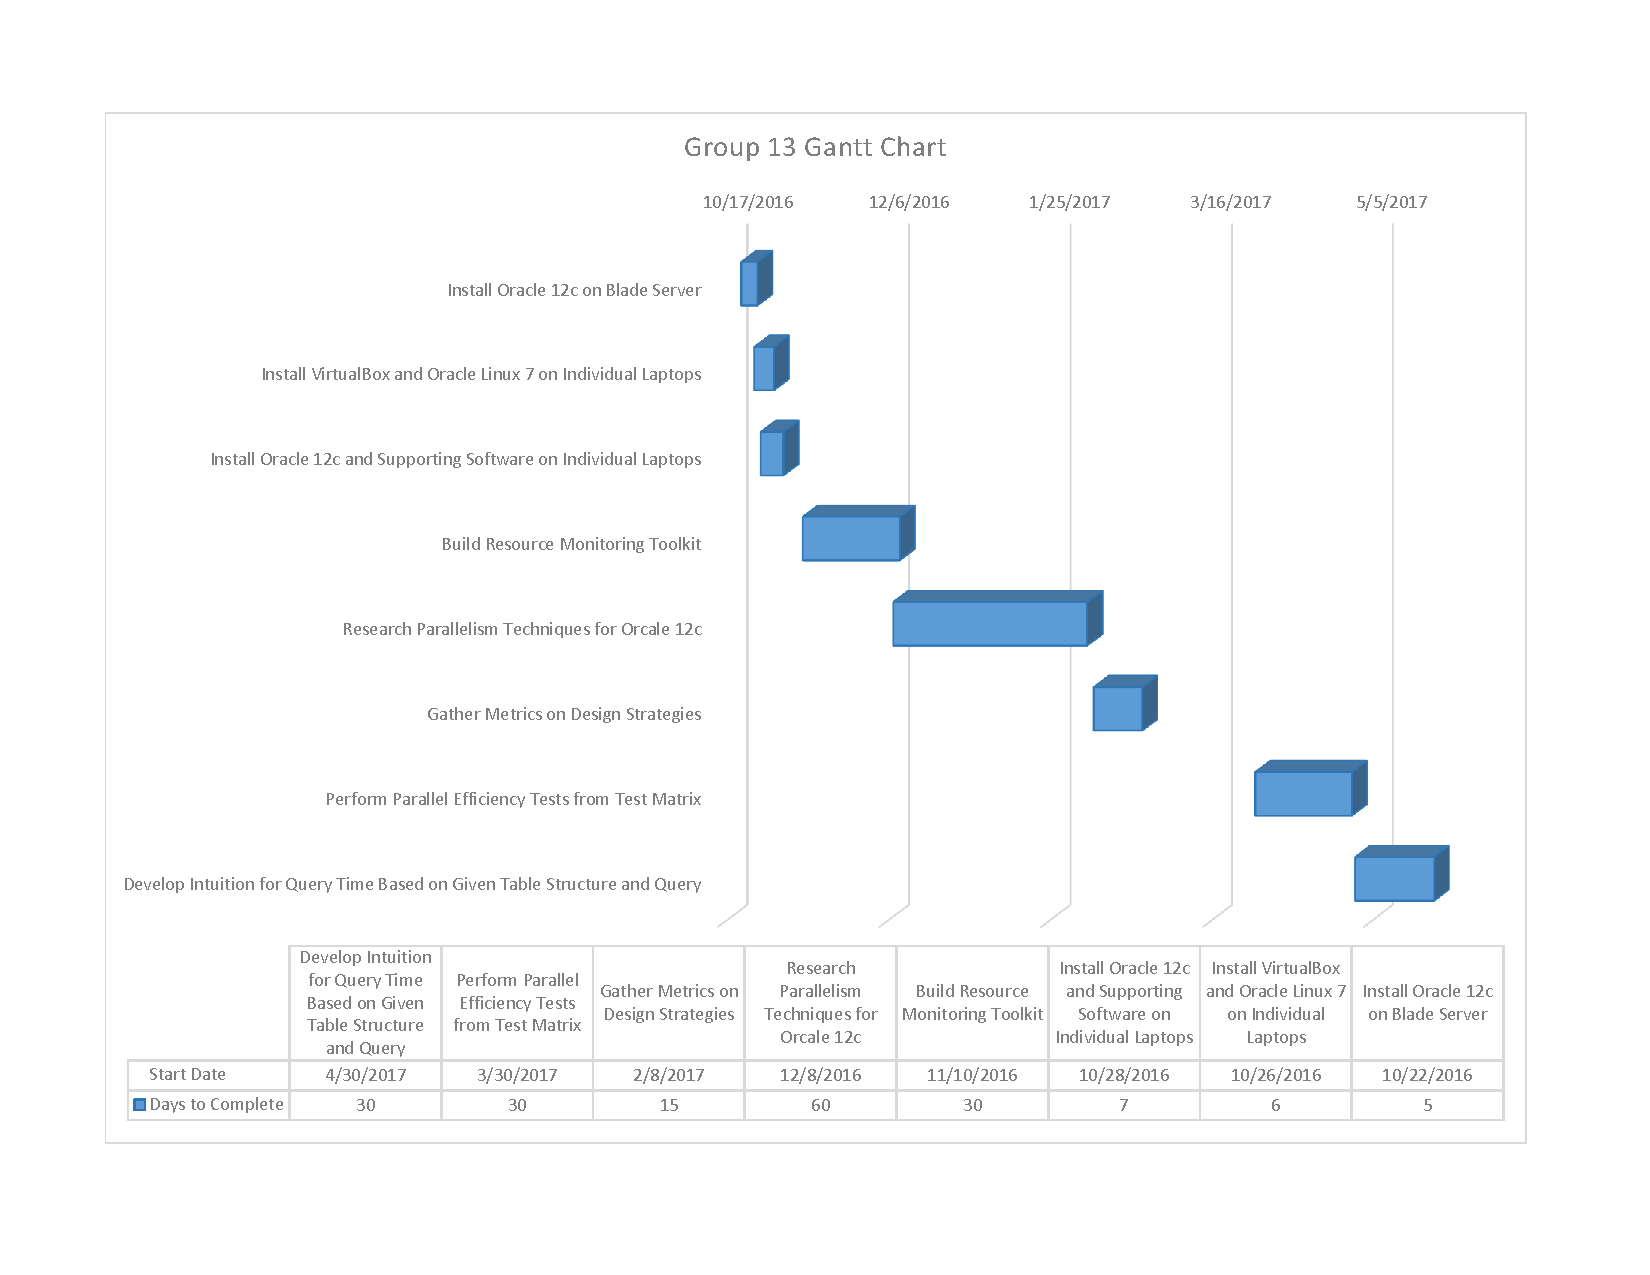
\includegraphics[width=\linewidth]{Gantt_Chart.pdf}

\end{document}